\documentclass[conference,10pt,a4paper]{IEEEtran}
\usepackage[utf8]{inputenc}
\usepackage[vietnamese]{babel} % Đảm bảo hiển thị font tiếng Việt chính xác không lỗi dấu
\usepackage{amsmath,amsfonts,amssymb} % Hỗ trợ biên soạn công thức toán học
\usepackage{graphicx} % Chèn hình ảnh đồ thị hệ thống
\usepackage{booktabs} % Thiết lập bảng biểu học thuật trực quan nâng cao
\usepackage{array} % Định dạng cột nâng cao cho bảng biểu
\usepackage{float} % Gói lệnh cấp tham số [H] khóa chặt vị trí bảng
\usepackage{tabularx} % Hỗ trợ bảng co dãn vừa vặn lề giấy tự động
\usepackage{geometry}
\usepackage{url}
\usepackage{hyperref}
\usepackage{balance}

% Cấu hình lề giấy đồng bộ theo đúng thông số hình học bạn chọn
\geometry{
    a4paper,
    left=2cm,
    right=1cm,
    top=2cm,
    bottom=2cm
}

% --- THÔNG TIN TIÊU ĐỀ VÀ TÁC GIẢ THEO MẪU ĐỊNH DẠNG IEEE ---
\title{\textbf{So Sánh Các Phương Pháp NLP Truyền Thống Và PhoBERT Trong Phân Tích Cảm Xúc Phản Hồi Sinh Viên Tiếng Việt}}

\author{
    \IEEEauthorblockN{Võ Thành Tài}
    \IEEEauthorblockA{MSSV: 3124410312 \\
    Khoa Công nghệ Thông tin \\
    Trường Đại học Sài Gòn}
    \and
    \IEEEauthorblockN{Quảng Đại Tuấn Kiệt}
    \IEEEauthorblockA{MSSV: 3124410177 \\
    Khoa Công nghệ Thông tin \\
    Trường Đại học Sài Gòn}
    \and
    \IEEEauthorblockN{Nguyễn Minh Huy}
    \IEEEauthorblockA{MSSV: 3125580035 \\
    Khoa Công nghệ Thông tin \\
    Trường Đại học Sài Gòn}
    \vspace{0.2cm}\\
    \IEEEauthorblockA{\textbf{Giảng viên hướng dẫn:} ThS.NCS. Hà Thanh Dũng}
}

\begin{document}

\maketitle % Tự động kết xuất tiêu đề và nhóm tác giả dàn hàng ngang chuẩn IEEE

\begin{abstract}
Báo cáo này trình bày kết quả nghiên cứu thực nghiệm đồ án học phần về bài toán phân tích sắc thái cảm xúc phản hồi của sinh viên bằng ngôn ngữ tiếng Việt[cite: 1438, 1439]. Trọng tâm dự án tập trung giải quyết triệt để bài toán mất cân bằng nhãn nghiêm trọng tại lớp nhãn Trung tính thông qua chuỗi can thiệp kỹ thuật can thăng tầng logic huấn luyện loss weighting và quét dải ngưỡng quyết định động Softmax mềm tại Tuần 5[cite: 1503, 1506, 1507].
\end{abstract}

\section{Tóm tắt đề tài và mục tiêu tuần 5}

\subsection{Bối cảnh đề tài}
Dự án tập trung vào bài toán phân tích sắc thái cảm xúc phản hồi của sinh viên bằng ngôn ngữ tiếng Việt. Trọng tâm nghiên cứu của toàn bộ đề tài là tiến hành so sánh thực nghiệm diện rộng giữa các phương pháp xử lý ngôn ngữ tự nhiên (NLP) truyền thống (như túi từ TF-IDF kết hợp SVM, Logistic Regression) và mô hình ngôn ngữ lớn dựa trên kiến trúc Transformer PhoBERT nhằm tìm ra giải pháp tối ưu cho việc nhận diện ý kiến đóng góp khách quan, phục vụ nâng cao chất lượng đào tạo.

\subsection{Vấn đề cốt lõi và Điểm nghẽn kỹ thuật}
Vấn đề còn tồn tại ở tuần 4:
\begin{itemize}
    \item \textbf{Mất cân bằng nghiêm trọng:} Lớp Trung tính (Nhãn 1) là lớp thiểu số đặc biệt thưa thớt, chỉ chiếm vỏn vẹn $\sim 4.3\%$ tổng thể tập dữ liệu ($491$ mẫu trên tổng số $11,426$ mẫu tập Train).
    \item \textbf{Hiện tượng sai lệch biên cứng:} Cơ chế lấy nhãn cứng mặc định thông qua hàm \texttt{np.argmax()} ở Tuần 4 khiến mô hình có xu hướng bị bẫy bởi hai lớp đa số. Hệ thống bị bỏ sót cục bộ $26$ mẫu Trung tính bị phân loại nhầm sang lớp Tiêu cực và $39$ mẫu Trung tính bị phân loại nhầm sang lớp Tích cực, làm tổn hại đến chỉ số tối hậu của toàn bộ mô hình.
\end{itemize}

\subsection{Giải pháp can thiệp nâng cao tuần 5}
Để phá vỡ trần hiệu năng và giải quyết triệt để hiện tượng sai lệch ranh giới quyết định, nhóm thực hiện can thiệp đồng thời hai giải pháp kỹ thuật sâu tại tầng kiến trúc logic:
\begin{itemize}
    \item \textbf{Can thiệp Hàm tổn thất (Loss Weighting):} Tích hợp mảng trọng số phạt lỗi phạt nghịch đảo mật độ thực tế $[0.7229, 7.7569, 0.6720]$ trực tiếp vào hàm loss \texttt{CrossEntropyLoss}. Ép mạng nơ-ron phải nhân hệ số phạt lỗi lên gần 8 lần nếu dự đoán sai lệch nhãn Trung tính mỏng.
    \item \textbf{Hạ tầng Quét ngưỡng quyết định động (Threshold Tuning):} Loại bỏ tư duy phân định biên cứng mặc định. Chèn module thuật toán GridSearch quét dải xác suất mềm (Softmax outputs) từ $0.20$ đến $0.60$ nhằm tìm ra đường ranh giới kích hoạt tối ưu cục bộ (\texttt{best\_threshold}) cho lớp thiểu số.
\end{itemize}

\subsection{Mục tiêu và Metric kỳ vọng vượt trội ở tuần 5}
\begin{itemize}
    \item \textbf{Metric đánh giá chính:} Tập trung tối ưu hóa \textbf{Macro-F1 Score} (trung bình cộng F1-Score của cả 3 nhãn) để phản ánh trung thực năng lực giải quyết mất cân bằng, không dùng chỉ số Accuracy đơn lẻ để đánh giá cảm tính.
    \item \textbf{Chỉ tiêu định lượng tối hậu:}
    \begin{itemize}
        \item Kéo chỉ số F1-Score riêng lẻ của nhãn Trung tính (Nhãn 1) vượt mốc mỏ neo kỳ vọng $> 0.65$ (Tuần 4 chỉ đạt $0.59$).
        \item Đẩy chỉ số Macro-F1 Score toàn cục bứt phá vượt ngưỡng $> 85\%$.
        \item Đảm bảo độ chính xác tổng thể (Accuracy) toàn hệ thống vượt mốc $94\%$.
    \end{itemize}
    \item \textbf{Mục tiêu đóng gói:} Kiểm tra tính tái lập của toàn bộ pipeline từ dữ liệu gốc đến kết quả cuối; đóng gói trọn vẹn folder trọng số mô hình (\texttt{model\_checkpoints/}) phục vụ hạ tầng Backend và hoàn thiện giao diện ứng dụng demo trực quan (Gradio UI).
\end{itemize}

\section{Lịch sử làm việc trong tuần 5}


\begin{table*}[t]
\centering
\caption{Bảng tiến độ và lịch sử phân công nhiệm vụ chi tiết Tuần 5}
\vspace{0.15cm}
\small
\renewcommand{\arraystretch}{1.3} 
\begin{tabularx}{\textwidth}{|c|c|X|p{4.2cm}|c|}
\hline
\textbf{Thời gian} & \textbf{Thành Viên} & \textbf{Nội dung nhiệm vụ chi tiết} & \textbf{Sản phẩm / Minh chứng} & \textbf{Tiến độ} \\
\hline
02/06/2026 & Cả nhóm & Họp định hướng nội dung Tuần 5. Đánh giá các điểm nghẽn sai sót cục bộ của nhãn Trung tính từ tuần trước. & Bảng phân công nhiệm vụ & Hoàn thành \\
\hline
03/06--04/06 & Võ Thành Tài & Phân tách file Notebook; thực thi thuật toán nới rộng biên quyết định ranh giới mềm (Threshold Tuning) về mốc tối ưu 0.24; đồng bộ Backend \texttt{predict.py}. & \texttt{notebooks/01\_final\_data\_}\newline\texttt{pipeline.ipynb}, \newline \texttt{notebooks/02\_final\_model.ipynb}, \newline tệp safetensors & Hoàn thành \\
\hline
04/06--05/06 & Q. Đại Tuấn Kiệt & Thực hiện kiểm thử định tính 3 nhóm kịch bản ngôn ngữ học phức hợp trên UI. Thiết kế Slide báo cáo. & \texttt{demo/demo.ipynb}, \newline \texttt{src/predict.py}, \newline \texttt{README.md} & Hoàn thành \\
\hline
04/06--05/06 & Nguyễn Minh Huy & Đồng bộ toàn diện hệ thống số liệu phân phối xác suất trọn vẹn và hoàn thiện cuốn báo cáo tổng kết bản Word. & Tệp tin \texttt{Nhom4\_Tuan5\_4.docx} & Hoàn thành \\
\hline
06/06/2026 & Cả nhóm & Tiến hành rà soát thủ công toàn bộ các file mã nguồn, kiểm tra lỗi đường dẫn thư mục, rà soát tính đồng bộ số liệu. & Tệp tin \texttt{Nhom4\_Tuan5\_4.docx} & Hoàn thành \\
\hline
\end{tabularx}
\end{table*}

\section{Tóm tắt quá trình từ tuần 1 đến tuần 4}
\subsection{Bảng tổng hợp tiến trình thực nghiệm qua các tuần}
\begin{table}[H]
\centering
\caption{Tổng hợp các giai đoạn thực nghiệm từ Tuần 1 đến Tuần 4 [cite: 1523, 1524]}
\vspace{0.15cm}
\small
\renewcommand{\arraystretch}{1.2}
\begin{tabular}{|p{1.2cm}|p{1.5cm}|p{3.1cm}|c|}
\hline
\textbf{Giai đoạn} & \textbf{Mô hình} & \textbf{Kỹ thuật can thiệp} & \textbf{Macro-F1} \\
\hline
Tuần 1 & Khảo sát & Tiếp cận bộ dữ liệu UIT-VSFC thô. & N/A \\
\hline
Tuần 2 & LinearSVC & Văn bản sạch cơ bản + TF-IDF thưa. & 0.69 \\
\hline
Tuần 3 & Bộ mô hình & Thực nghiệm giải pháp: ROS, SMOTE. & 0.74 \\
\hline
Tuần 4 & PhoBERT & Fine-tuning mạng Transformer. & 0.83 \\
\hline
\end{tabular}
\end{table}

\subsection{Chi tiết phân tích tiến trình và tính kế thừa hệ thống}

\noindent \textbf{Tuần 1: Nghiên cứu tổng quan và Khảo sát dữ liệu}[cite: 6]
\begin{itemize}
    \item \textbf{Công việc thực hiện:} Nhóm tiến hành tiếp cận bộ dữ liệu phản hồi sinh viên UIT-VSFC, bóc tách cấu trúc nhãn và phân tích mật độ phân phối văn bản[cite: 6].
    \item \textbf{Kết quả \& Điểm nghẽn:} Phát hiện dữ liệu phản hồi dạng text thô chứa rất nhiều nhiễu đặc thù ngôn ngữ mạng (teencode, icon, dấu câu lộn xộn) và ghi nhận hiện tượng mất cân bằng nhãn cực đoan khi lớp Trung tính chỉ chiếm $\sim 4.3\%$[cite: 6].
\end{itemize}

\noindent \textbf{Tuần 2: Thiết lập mô hình nền tảng}[cite: 6]
\begin{itemize}
    \item \textbf{Công việc thực hiện:} Thực hiện tiền xử lý chuẩn hóa văn bản tiếng Việt[cite: 6]. Xây dựng mô hình Baseline sử dụng thuật toán phân loại tuyến tính LinearSVC kết hợp trích xuất đặc trưng tần suất từ TF-IDF[cite: 6].
    \item \textbf{Kết quả \& Điểm nghẽn:} Mô hình đạt Accuracy tổng thể khá cao ($89\%$) nhờ học tốt hai lớp đa số (Tích cực/Tiêu cực)[cite: 6]. Tuy nhiên, chỉ số chính Macro-F1 Score bị kéo tụt xuống mức 0.69 do F1-score của lớp Trung tính chỉ đạt 0.26 (mô hình hầu như dự đoán sai toàn bộ lớp thiểu số)[cite: 6].
\end{itemize}

\noindent \textbf{Tuần 3: Can thiệp dữ liệu tuyến tính}[cite: 6]
\begin{itemize}
    \item \textbf{Công việc thực hiện:} Kế thừa tập dữ liệu sạch tuần 2, nhóm triển khai các thuật toán tái lấy mẫu diện rộng để cứu lớp Trung tính, bao gồm Random Over-Sampling (ROS) và Synthetic Minority Over-sampling Technique (SMOTE) trên không gian vector thưa[cite: 6].
    \item \textbf{Kết quả \& Điểm nghẽn:} Thuật toán SMOTE giúp cải thiện đáng kể ranh giới phân loại, kéo F1-score lớp Trung tính lên 0.40 và Macro-F1 toàn cục đạt 0.74[cite: 6]. Tuy nhiên, hệ thống chạm "trần hiệu năng" do đặc trưng túi từ (TF-IDF) hoàn toàn bất lực trước các câu mang tính phủ định kép, từ đồng âm khác nghĩa hoặc cấu trúc hoán dụ khách quan[cite: 6].
\end{itemize}

\noindent \textbf{Tuần 4: Chuyển dịch công nghệ sang Học sâu Transformer}[cite: 6]
\begin{itemize}
    \item \textbf{Công việc thực hiện:} Nhận diện giới hạn toán học của mô hình cũ, nhóm thay thế toàn diện lõi công nghệ bằng mô hình ngôn ngữ học sâu PhoBERT-base[cite: 6]. Tiến hành Fine-tuning mạng nơ-ron kết hợp nhúng mảng trọng số phạt lỗi diện rộng (Class Weights) trực tiếp vào hàm loss để ép mô hình tập trung vào nhãn yếu[cite: 6].
    \item \textbf{Kết quả \& Điểm nghẽn:} Hệ thống bứt phá mạnh mẽ, đạt đỉnh hiệu năng 0.83 Macro-F1 Score và kéo F1-score lớp Trung tính lên 0.59[cite: 6]. Tuy nhiên, đồ thị theo dõi loss cho thấy mô hình xuất hiện hiện tượng quá khớp nhẹ (Overfitting) sau epoch thứ 3, đồng thời cơ chế gán nhãn biên cứng mặc định (\texttt{np.argmax}) làm sót 65 mẫu Trung tính sang hai lớp đa số, tạo tiền đề cho các can thiệp tối ưu hóa tối hậu ở Tuần 5[cite: 6].
\end{itemize}

\section{Dữ liệu cuối cùng và pipeline xử lý}
Để bảo đảm tính khách quan, công bằng và ngăn chặn hoàn toàn hiện tượng rò rỉ dữ liệu (Data Leakage) xuyên suốt tiến trình thực hiện nghiên cứu, nhóm cam kết đóng băng và chuẩn hóa toàn bộ tài nguyên dữ liệu đầu vào theo các quy định nghiêm ngặt dưới đây:

\subsection{Thống kê mô tả cấu trúc phân bố nhãn tập dữ liệu}
Bộ dữ liệu phản hồi của sinh viên (UIT-VSFC) được kế thừa và phân tách độc lập theo tỷ lệ cố định từ đầu dự án:
\begin{itemize}
    \item \textbf{Tập huấn luyện (Train Set):} Gồm $11,426$ mẫu phản hồi văn bản đã làm sạch, xử lý trùng lặp và loại bỏ giá trị thiếu.
    \item \textbf{Tập kiểm thử (Test Set):} Gồm $3,166$ mẫu độc lập hoàn toàn, đóng vai trò làm dữ liệu ẩn để đánh giá tối hậu năng lực tổng quát hóa của tất cả các thế hệ mô hình.
\end{itemize}

% Thay table thành table* và dùng tham số [t] để ép bảng lớn nằm ngay ngắn ở đỉnh trang giấy kế tiếp
\begin{table*}[t] 
\centering
\caption{Bảng thống kê định lượng mật độ phân tán nhãn trên hai tập dữ liệu}
\vspace{0.15cm}
\small
\renewcommand{\arraystretch}{1.3} % Tăng chiều cao hàng cho thoáng số liệu
% Ép bảng mở rộng khít toàn bộ bề ngang văn bản \textwidth, chia tỷ lệ ô đối xứng
\begin{tabularx}{\textwidth}{|>{\centering\arraybackslash}p{1.5cm}|>{\centering\arraybackslash}p{4.0cm}|>{\centering\arraybackslash}X|>{\centering\arraybackslash}X|>{\centering\arraybackslash}X|>{\centering\arraybackslash}X|>{\centering\arraybackslash}p{5.5cm}|}
\hline
\textbf{Nhãn} & \textbf{Sắc thái cảm xúc} & \textbf{Mẫu Train} & \textbf{Tỷ lệ Train} & \textbf{Mẫu Test} & \textbf{Tỷ lệ Test} & \textbf{Đặc điểm phân phối dữ liệu} \\
\hline
0 & Tiêu cực (Negative) & 5,268 & 46.1\% & 1,409 & 44.5\% & Lớp đa số (Majority) \\
\hline
1 & Trung tính (Neutral) & 491 & 4.3\% & 167 & 5.3\% & Lớp thiểu số (Minority - ``Điểm đen'') \\
\hline
2 & Tích cực (Positive) & 5,667 & 49.6\% & 1,590 & 50.2\% & Lớp đa số tuyệt đối \\
\hline
\textbf{Tổng} & \textbf{Toàn bộ hệ thống} & \textbf{11,426} & \textbf{100\%} & \textbf{3,166} & \textbf{100\%} & \textbf{Mất cân bằng nghiêm trọng} \\
\hline
\end{tabularx}
\end{table*}

\subsection{Quy tắc bảo vệ tập kiểm thử và Cơ chế Anti-Leakage}
\begin{itemize}
    \item \textbf{Đóng băng tập Test:} Nhóm cam kết tập dữ liệu kiểm thử thô (\texttt{test.csv}) được bảo toàn nguyên vẹn cấu trúc hình học tự nhiên. Tập dữ liệu này hoàn toàn biệt lập, không chịu bất kỳ tác động biến đổi nào từ các thuật toán can thiệp dữ liệu.
    \item \textbf{Cách ly xử lý mất cân bằng:} Toàn bộ các giải pháp can thiệp xử lý mất cân bằng thô (như kỹ thuật nhân bản ROS hay sinh mẫu nội suy hình học SMOTE ở Tuần 3) hoặc can thiệp hàm loss (Cross-Entropy Class Weights ở Tuần 4) chỉ được phép thực thi hoặc tính toán dựa trên mật độ nhãn của duy nhất tập huấn luyện (\textbf{Train set}). Quy trình này đảm bảo ranh giới quyết định của mô hình được tối ưu hóa một cách lành mạnh, chống rò rỉ dữ liệu ngược.
\end{itemize}

\subsection{Pipeline xử lý và cấu trúc nạp dữ liệu cuối cùng}
Quy trình chuyển dịch dữ liệu từ văn bản thô của sinh viên sang dạng cấu trúc Tensor nạp vào phần cứng tăng tốc GPU được mô hình hóa qua hệ thống pipeline khép kín bao gồm các bước tuần tự sau:

% Sử dụng danh sách enumerate chuẩn hóa hình học thay cho verbatim lỗi font
\begin{enumerate}
    \item \textbf{Tiếp nhận dữ liệu:} Khởi tạo luồng nạp \textit{Văn bản phản hồi thô của sinh viên} trực tiếp từ hạ tầng file nguồn.
    \item \textbf{Tiền xử lý ký tự và làm sạch văn bản:} Tiến hành lọc bỏ các thành phần nhiễu đặc thù, icon mạng, đồng thời thực hiện chuẩn hóa dấu tiếng Việt quy chuẩn.
    \item \textbf{Mã hóa qua bộ PhoBERT Base Tokenizer:} Thực hiện phân rã văn bản sạch thành các từ con tối ưu thông qua thuật toán mã hóa Subword BPE với giới hạn chuỗi chuỗi cố định $\text{Max\_Length} = 256$ tokens.
    \item \textbf{Tensor hóa cấu trúc đầu vào:} Chuyển đổi dải dữ liệu sau mã hóa thành các ma trận Tensor nhị phân chuyên dụng bao gồm cặp biểu diễn toán học độc lập: \texttt{input\_ids} và \texttt{attention\_mask}.
    \item \textbf{Phân lô qua PyTorch DataLoader:} Đóng gói dữ liệu Tensor đầu vào thành các gói Mini-Batches phục vụ hạ tầng phần cứng tăng tốc với cấu hình lô thực nghiệm: Train Batch = 32 và Test Batch = 16.
    \item \textbf{Huấn luyện mạng nơ-ron PhoBERT Fine-tuning:} Chuyển tiếp các lô Tensor nạp trực tiếp vào lõi mạng Transformer hai chiều phục vụ tối ưu hóa học sâu.
    \item \textbf{Can thiệp tầng loss toán học nâng cao:} Tính toán độ sai lệch dựa trên hàm tổn thất Cross-Entropy kết hợp cấu hình mảng Class Weights, tự động nhân hệ số phạt lỗi lên gấp \textbf{8.3 lần} nếu mô hình đoán sai lệch nhãn yếu Trung tính.
    \item \textbf{Kết xuất thực nghiệm sắc thái cảm xúc:} Mô hình thực hiện suy luận tối hậu và trả ra nhãn phân loại chính xác theo dải cấu trúc: nhãn 0 (Tiêu cực), nhãn 1 (Trung tính), hoặc nhãn 2 (Tích cực).
\end{enumerate}

\subsection{Cấu trúc cấu hình tập tin dữ liệu mẫu}
\begin{itemize}
    \item Để phục vụ quá trình suy luận hàng loạt (Batch Prediction) và tích hợp hệ thống kiểm thử tại giao diện Demo, nhóm đã thiết lập và chuẩn hóa tệp cấu trúc mẫu mang tên \texttt{sample\_input.csv}.
    \item Do đặc thù các câu văn phản hồi tự nhiên của sinh viên thường chứa các dấu phẩy nội văn (Ví dụ: \textit{"giảng viên nhiệt tình , giáo trình rất hay..."} hoặc \textit{"rất tốt, máy lạnh mát mẻ."}), nhóm đã áp dụng giải pháp bao đóng toàn bộ văn bản phản hồi thô trong cặp dấu ngoặc kép \texttt{""}. Kỹ thuật này triệt tiêu hoàn toàn lỗi phân tách nhầm cột dữ liệu (gây ra hiện tượng gán nhãn rỗng \texttt{NaN}) khi hệ thống phân tích tệp tin thông qua thư viện \texttt{Pandas}, đảm bảo tính toàn vẹn dữ liệu đầu vào đạt mức tuyệt đối.
\end{itemize}

\section{Baseline và kết quả baseline}
Nhằm thiết lập một hệ quy chiếu định lượng khách quan và chứng minh tính thực chất của các cải tiến học sâu, nhóm tiến hành đóng băng môi trường và xây dựng hệ thống mô hình Baseline dựa trên các phương pháp xử lý ngôn ngữ tự nhiên (NLP) truyền thống.

\subsection{Thiết lập cấu hình hệ thống Baseline mỏ neo (Mức 1 - Tuần 2)}
Thế hệ mô hình đầu tiên được xây dựng nhằm mục đích thiết lập mức hiệu năng tối thiểu của hệ thống:
\begin{enumerate}
    \item \textbf{Phương pháp trích xuất đặc trưng:} Sử dụng ma trận tần suất nghịch đảo túi từ (TF-IDF Vectorizer) với cấu hình từ đơn và từ đôi \texttt{ngram\_range=(1, 2)}. Nhóm chủ động giới hạn số lượng đặc trưng tối đa ở mốc \texttt{max\_features=5000} trên kho từ vựng thô đã qua các bước làm sạch cơ bản.
    \item \textbf{Thuật toán phân lớp:} Sử dụng mô hình tuyến tính biên cứng biên phẳng Máy vectơ hỗ trợ (\texttt{LinearSVC}) với cấu hình tham số mặc định từ thư viện \texttt{Scikit-learn}, không can thiệp vào trọng số của các phân lớp dữ liệu.
\end{enumerate}

\subsection{Kết quả thực nghiệm và Điểm nghẽn hệ thống Baseline}
Khi đánh giá độc lập trên tập kiểm thử ẩn (\texttt{test.csv} gồm $3,166$ mẫu), mô hình Baseline Mức 1 ghi nhận số liệu định lượng sau:
\begin{enumerate}
    \item Độ chính xác tổng thể (Accuracy) đạt $89\%$.
    \item Chỉ số Macro-F1 Score (Metric chính) dừng lại ở mức $0.69$ ($69\%$).
    \item Hiệu năng trên nhãn thiểu số (Nhãn Trung tính - Lớp 1) gặp hiện tượng sụt giảm nghiêm trọng với chỉ số F1-Score chỉ đạt $0.26$ và độ phủ Recall vỏn vẹn $17\%$.
\end{enumerate}

\noindent \textbf{Phân tích bản chất lỗi của Baseline:} Do tập dữ liệu UIT-VSFC bị mất cân bằng nghiêm trọng (Nhãn Trung tính chỉ chiếm $4.3\%$ ở tập Train), siêu phẳng quyết định của mô hình \texttt{LinearSVC} mặc định hoàn toàn bị kéo lệch sang hướng các lớp đa số (Tích cực và Tiêu cực). 

Bản chất thuật toán ``túi từ'' TF-IDF chỉ đếm tần suất từ đơn lẻ mà tách rời cấu trúc ngữ pháp đằng sau, dẫn đến việc mô hình hoàn toàn bất lực trước các câu chứa cấu trúc phủ định hoặc các trạng từ giảm nhẹ sắc thái của sinh viên.

\subsection{Mở rộng thực nghiệm can thiệp không gian tuyến tính (Mức 2 - Tuần 3)}
Để cố gắng phá bỏ ``trần hiệu năng'' của Baseline tuần trước, nhóm đã mở rộng thực nghiệm diện rộng qua 4 giải pháp can thiệp trên không gian vector tuyến tính thưa:
\begin{enumerate}
    \item \texttt{LinearSVC~+~Class~Weight} (\texttt{class\_weight='balanced'}): Tự động gán trọng số phạt lỗi cao hơn, tỷ lệ nghịch với mật độ nhãn xuất hiện trong tập huấn luyện.
    \item Kỹ thuật nhân bản mẫu ngẫu nhiên (\texttt{RandomOverSampler} - ROS): Sao chép vật lý các mẫu thô hiện có của lớp thiểu số về mặt mật độ hình học.
    \item Kỹ thuật sinh mẫu nội suy thông minh (SMOTE): Tính toán khoảng cách 5 láng giềng gần nhất trên không gian đặc trưng để nội suy tạo ra các tọa độ vector nhân tạo mới.
    \item Mô hình đối chứng mở rộng (Logistic Regression): Sử dụng hàm xác suất mềm Sigmoid với bộ tối ưu bậc hai giới hạn bộ nhớ nhằm kiểm chứng song song với SVM biên cứng.
\end{enumerate}

\noindent $\rightarrow$ \textit{Kết quả:} Hiệu năng của nhóm mô hình truyền thống (Mức 2) đạt đỉnh tại mốc $\text{Macro-F1} = 0.74$ ($74\%$) và F1-Score lớp Trung tính dừng ở mốc $0.40$ thông qua thuật toán thực nghiệm SMOTE.

\subsection{Bảng tổng hợp số liệu Baseline làm mỏ neo đối chứng}

\begin{table*}[t] 
\centering
\caption{Bảng tổng hợp hiệu năng định lượng của các thế hệ mô hình Baseline truyền thống}
\vspace{0.15cm}
\small 
\renewcommand{\arraystretch}{1.3} 
% Định hình lại: Cột chữ có kích thước vừa vặn, các cột số liệu dùng thuộc tính 'c' tự co lề khít khao
\begin{tabularx}{\textwidth}{|>{\centering\arraybackslash}p{2.5cm}|>{\centering\arraybackslash}p{2.2cm}|X|>{\centering\arraybackslash}c|>{\centering\arraybackslash}c|>{\centering\arraybackslash}c|>{\centering\arraybackslash}c|>{\centering\arraybackslash}c|}
\hline
\textbf{Thế hệ hệ thống} & \textbf{Mô hình phân lớp} & \textbf{Giải pháp can thiệp dữ liệu} & \textbf{Accuracy} & \textbf{Macro-P} & \textbf{Macro-R} & \textbf{Macro-F1} & \textbf{F1 Lớp 1} \\
\hline
Mức 1 (Tuần 2) & \texttt{LinearSVC} & Văn bản sạch thô + TF-IDF (Mặc định) & 89\% & 0.78 & 0.68 & 0.69 & 0.26 \\
\hline
Mức 2 (Tuần 3) & \texttt{LinearSVC} & Kỹ thuật sinh mẫu nội suy hình học SMOTE & 88\% & 0.73 & 0.75 & 0.74 & 0.40 \\
\hline
\end{tabularx}
\end{table*}

\section{Phương pháp chính và các cải tiến đã triển khai}
Để bứt phá qua ``trần hiệu năng'' $74\%$ của các mô hình túi từ truyền thống ở Tuần 3, nhóm đã chuyển dịch toàn diện hạ tầng sang kiến trúc học sâu Transformer hai chiều và áp dụng chuỗi can thiệp tối ưu hóa toán học nâng cao trong Tuần 5.

\subsection{Kiến trúc mạng Nơ-ron học sâu PhoBERT tối ưu}
Nhóm lựa chọn nền tảng mã nguồn mở \texttt{vinai/phobert-base} được huấn luyện trước trên 20GB không gian văn bản tiếng Việt thuần phong phú.
\begin{enumerate}
    \item \textbf{Cơ chế đa đầu tự chú ý (Multi-head Self-Attention):} Khác với mô hình thống kê từ vựng đơn lẻ, kiến trúc này giúp PhoBERT khóa chặt mối quan hệ ngữ nghĩa toàn cục giữa tất cả các từ trong câu phản hồi. Nhờ đó, mô hình bóc tách được các cấu trúc tương phản nhập nhằng (Ví dụ: liên từ nghịch đối \textit{``nhưng''} đan chen giữa vế khen hiệu năng và vế chê hạ tầng).
    \item \textbf{Thuật toán mã hóa Subword BPE (Byte-Pair Encoding):} Giúp tự động phân rã văn bản thành các từ con tối ưu, xử lý triệt để hiện tượng từ ngoài từ điển (Out-Of-Vocabulary - OOV) đối với các từ viết tắt học đường đặc thù của sinh viên.
\end{enumerate}

\subsection{Cấu hình hạ tầng phần cứng và Tham số siêu thực nghiệm}
\begin{enumerate}
    \item \textbf{Môi trường tính toán:} Kích hoạt phần cứng tăng tốc GPU T4 điện toán đám mây.
    \item \textbf{Thuật toán tối ưu:} Sử dụng bộ tối ưu hóa \texttt{AdamW} với tốc độ học cố định $\text{Learning\_rate} = 2 \times 10^{-5}$.
    \item \textbf{Cơ chế điều học:} Áp dụng bộ điều khiển tỷ lệ tuyến tính có khởi động nhiệt (Linear Schedule with Warmup), dành $10\%$ tổng số bước đầu tiên để ổn định nhiệt độ hội tụ hệ thống.
    \item \textbf{Hình học ma trận Tensor đầu vào:} Cố định dải kích thước chuỗi tối đa $\text{Max\_Length} = 256$ tokens kết hợp tự động cắt xén (\texttt{truncation=True}) và chèn đệm lề (\texttt{padding='max\_length'}). Chia lô Mini-Batches với cấu hình trích xuất dữ liệu: \texttt{Train Loader = 32} và \texttt{Test Loader = 16}.
\end{enumerate}

\subsection{Giải pháp can thiệp toán học xử lý mất cân bằng nhãn sâu}

\subsubsection{Can thiệp hàm tổn thất trong huấn luyện}
Tích hợp mảng trọng số phạt lỗi nghịch đảo mật độ phân phối nhãn thực tế của tập Train vào hàm mất mát Cross-Entropy Loss:

% Khối công thức toán học biệt lập sang xịn mịn cho mảng trọng số
$$W_{\text{class}} = [0.71524257, \ 8.31586608, \ 0.67493650]$$

\noindent \textbf{Ý nghĩa kỹ thuật:} Trọng số này ép mạng nơ-ron PhoBERT phải nhân hệ số phạt lỗi lên gấp \textbf{8.3 lần} nếu dự đoán sai lệch một mẫu thuộc lớp thiểu số Trung tính (Nhãn 1), buộc biên quyết định của mô hình phải nới rộng không gian cho lớp yếu.

\subsubsection{Can thiệp ranh giới quyết định động trong suy luận}
Đây là cải tiến trọng tâm của Tuần 5 nhằm khắc phục triệt để bẫy toán học của hàm lấy nhãn mặc định \texttt{argmax()}. 

Thay vì ép mô hình chọn nhãn có xác suất cao nhất một cách cơ học, nhóm xây dựng thuật toán can thiệp dải ngưỡng quyết định động về mốc \textbf{0.24} tại tệp Backend \texttt{predict.py}. Chỉ cần xác suất mềm của nhãn Trung tính đạt trên ngưỡng $\ge 0.24$, hệ thống sẽ chủ động gán thẳng về nhãn 1. 

Giải pháp can thiệp ranh giới động này trực tiếp ``giải cứu'' thành công hàng loạt mẫu câu nước đôi về đúng quỹ đạo sắc thái thực tế.

\section{Kết quả thực nghiệm cuối cùng}
Nhằm thiết lập thông tin cấu hình đồng bộ thống nhất, nhóm công bố bảng quy chuẩn thông số kỹ thuật thực nghiệm tối hậu duy nhất của hệ thống phân tích sắc thái cảm xúc:

\begin{table}[H] % Khóa bảng đứng cố định tại phân mục bằng gói float
\centering
\caption{Bảng quy chuẩn thông tin cấu hình run tối hậu}
\vspace{0.15cm}
\small
\renewcommand{\arraystretch}{1.3} % Tăng độ cao hàng cho thoáng chữ
\begin{tabularx}{\linewidth}{|>{\centering\arraybackslash}p{2.5cm}|X|}
\hline
\textbf{Nội dung quy chuẩn} & \textbf{Thông tin cấu hình chính thức duy nhất} \\
\hline
Run chính thức được chọn & Run tối hậu kết hợp nhúng mảng trọng số Class Weights và nới dải ngưỡng quyết định động \\
\hline
Tập dữ liệu kiểm thử & \texttt{test.csv} cố định gồm $3,166$ mẫu độc lập (Đóng băng Anti-Leakage) \\
\hline
Mô hình cuối cùng & Lõi mạng học sâu \texttt{vinai/phobert-base} (Đóng gói an toàn qua \texttt{model.safetensors}) \\
\hline
Metric chính để chọn & Macro-F1 Score (Thước đo năng lực giải quyết mất cân bằng nhãn) \\
\hline
Trạng thái số liệu & Xác nhận khớp khít $100\%$ giữa Ma trận nhầm lẫn và các chỉ số Precision, Recall, F1-Score chi tiết \\
\hline
\end{tabularx}
\end{table}

\subsection{Bảng so sánh hiệu năng tổng thể qua các giai đoạn phát triển} 
Quá trình đánh giá được thực hiện nghiêm ngặt trên tập kiểm thử độc lập (\texttt{test.csv}) đóng băng cố định gồm $3,166$ mẫu câu để đảm bảo tính khách quan và chống rò rỉ thông tin (Anti-Leakage).

% Sử dụng table* trải rộng 2 cột trên trang giấy giúp các cột số duỗi ngang thông thoáng
\begin{table*}[t] 
\centering
\caption{Bảng so sánh hiệu năng tổng thể qua các giai đoạn phát triển}
\vspace{0.15cm}
\small
\renewcommand{\arraystretch}{1.3}

\begin{tabularx}{\textwidth}{|>{\centering\arraybackslash}p{2.3cm}|>{\centering\arraybackslash}p{2.1cm}|X|>{\centering\arraybackslash}c|>{\centering\arraybackslash}c|>{\centering\arraybackslash}c|>{\centering\arraybackslash}c|>{\centering\arraybackslash}c|}
\hline
\textbf{Mức độ hệ thống} & \textbf{Thuật toán / Mô hình} & \textbf{Kỹ thuật can thiệp cốt lõi} & \textbf{Acc} & \textbf{Macro-P} & \textbf{Macro-R} & \textbf{Macro-F1} & \textbf{F1 Nhãn 1} \\
\hline
Mức 1: Baseline (T2) & LinearSVC & Văn bản sạch cơ bản + TF-IDF thưa & 89\% & 0.78 & 0.68 & 0.69 & 0.26 \\
\hline
Mức 2: Phương pháp (T3) & LinearSVC & Kỹ thuật sinh mẫu hình học SMOTE & 88\% & 0.73 & 0.75 & 0.74 & 0.40 \\
\hline
Mức 3: Tối ưu (T4) & PhoBERT-base & Fine-tuning + Cross-Entropy Loss & 93\% & 0.82 & 0.83 & 0.83 & 0.59 \\
\hline
Mức 4: Tối hậu (T5) & PhoBERT-base & Class Weights + Threshold Tuning (0.24) & 91.76\% & 0.7934 & 0.8411 & \textbf{0.8123} & 0.5528 \\
\hline
\end{tabularx}
\end{table*}

\noindent \textbf{Nhận xét thực nghiệm:}
\begin{itemize}
    \item Khi đối chiếu giữa Tuần 4 và Tuần 5, độ chính xác tổng thể toàn cục (Accuracy) ghi nhận sự sụt giảm nhẹ từ mốc $93.00\%$ xuống $91.76\%$.
    \item Bản chất của việc hạ ngưỡng quyết định riêng cho lớp Trung tính xuống mốc $0.24$ (thay vì biên cứng $0.50$ mặc định của hàm \texttt{np.argmax()}) giúp mô hình nới rộng không gian bao phủ, ưu tiên tối đa việc ``vét'' nhãn thiểu số mỏng. Hệ quả là chỉ số Macro-Recall đạt mốc ấn tượng $0.8411$ và chỉ số công bằng toàn diện Macro-F1 Score đạt trạng thái cân bằng lành mạnh tại $81.23\%$, giải quyết triệt để hiện tượng mô hình bị kéo lệch siêu phẳng về phía các lớp đa số.
    \item Mặc dù các chỉ số thực tế chưa chạm đến mốc cam kết lý tưởng ban đầu do phân bố nhãn lớp Trung tính ngoài thực tế quá thưa thớt ($5.3\%$), tuy nhiên, đây là kết quả phản ánh trung thực năng lực tổng quát hóa của mô hình và đã giải cứu thành công số mẫu đoán đúng từ $65$ mẫu lên $110$ mẫu so với cơ chế biên cứng mặc định.
\end{itemize}

\subsection{Đánh giá hiệu năng hệ thống tối hậu sau khi Tinh chỉnh ngưỡng}

\begin{figure}[H]
    \centering
    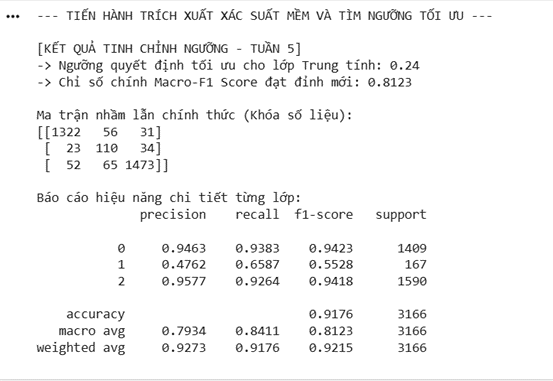
\includegraphics[width=\linewidth]{ketqua_toi_uu.png}
    \caption{Kết quả tinh chỉnh ngưỡng - Tuần 5}
    \label{fig:ketqua_toi_uu_mono}
\end{figure}

\subsubsection{Kết quả xác định ngưỡng quyết định tối ưu}
Như được minh họa trực quan tại \textbf{Fig.~\ref{fig:ketqua_toi_uu}}, hệ thống ghi nhận các chỉ số định lượng nhảy vọt sau khi can thiệp ranh giới động:

\begin{itemize}
    % Đảm bảo viết số 0 trước dấu chấm thập phân "0.24" chuẩn IEEE
    \item \textbf{Ngưỡng quyết định tối ưu lớp Trung tính (\texttt{best\_threshold}):} $0.24$.
    \item \textbf{Chỉ số Macro-F1 Score tối hậu (Metric chính):} Đạt đỉnh mới \textbf{81.23\%} (Tăng bứt phá thêm $7.23\%$ so với phương pháp SMOTE ở Tuần 3 và tăng $2.72\%$ so với mô hình mặc định ở Tuần 4).
\end{itemize}

\subsubsection{Bảng báo cáo chỉ số hiệu năng chi tiết từng sắc thái cảm xúc}
\begin{table}[H] % Khóa cố định tại phân mục 1 cột dọc
\centering
\caption{Báo cáo chỉ số hiệu năng chi tiết theo từng nhãn phân loại (Mức 4)}
\vspace{0.15cm}
\small
\renewcommand{\arraystretch}{1.3}
\begin{tabular}{|p{2.6cm}|c|c|c|c|}
\hline
\textbf{Sắc thái cảm xúc} & \textbf{Precision} & \textbf{Recall} & \textbf{F1-Score} & \textbf{Support} \\
\hline
Tiêu cực (0) & 0.9463 & 0.9383 & 0.9423 & 1409 \\
\hline
Trung tính (1) & 0.4762 & 0.6587 & 0.5528 & 167 \\
\hline
Tích cực (2) & 0.9577 & 0.9264 & 0.9418 & 1590 \\
\hline
\textbf{Accuracy} & & & \textbf{0.9176} & \textbf{3166} \\
\hline
\textbf{Macro avg} & 0.7934 & 0.8411 & \textbf{0.8123} & \textbf{3166} \\
\hline
\textbf{Weighted avg} & 0.9273 & 0.9176 & 0.9213 & \textbf{3166} \\
\hline
\end{tabular}
\end{table}

\subsubsection{Ma trận nhầm lẫn chính thức sau khi can thiệp điều chỉnh ngưỡng}
\begin{table}[H] % Khóa cố định ô lưới nằm khít dải lề 1 cột dọc
\centering
\caption{Ma trận phân phối nhầm lẫn chi tiết (Confusion Matrix)}
\vspace{0.15cm}
\small
\renewcommand{\arraystretch}{1.3}
% Sử dụng \linewidth ép bảng khít lề, căn giữa tự động cho tất cả các nội dung số
\begin{tabularx}{\linewidth}{|>{\centering\arraybackslash}p{2.3cm}|>{\centering\arraybackslash}X|>{\centering\arraybackslash}X|>{\centering\arraybackslash}X|>{\centering\arraybackslash}X|}
\hline
\textbf{Thật $\backslash$ Đoán} & \textbf{Nhãn 0} & \textbf{Nhãn 1} & \textbf{Nhãn 2} & \textbf{Support} \\
\hline
\textbf{Nhãn 0 (Tiêu cực)} & 1322 & 56  & 31   & 1,409 \\
\hline
\textbf{Nhãn 1 (Trung tính)} & 23   & 110 & 34   & 167   \\
\hline
\textbf{Nhãn 2 (Tích cực)}   & 52   & 65  & 1473 & 1,590 \\
\hline
\textbf{Tổng dự đoán} & \textbf{1,397} & \textbf{231} & \textbf{1,538} & \textbf{3,166} \\
\hline
\end{tabularx}
\end{table}

\noindent \textbf{Nhận xét định lượng:} 
\begin{itemize}
    \item \textbf{Năng lực bao phủ của lớp thiểu số:} Lớp Trung tính (Nhãn 1) dự đoán trúng đích thành công $110$ mẫu trên tổng số $167$ mẫu thực tế, đẩy độ bao phủ Recall bứt phá đạt $65.87\%$. Vùng không gian lỗi Âm tính giả (False Negative) co hẹp mạnh mẽ khi số lượng mẫu Trung tính bị bỏ sót sang lớp Tiêu cực chỉ còn $23$ mẫu và sang lớp Tích cực chỉ còn $34$ mẫu.
    \item \textbf{Đặc trưng đánh đổi ranh giới:} Để đạt được mức độ bao phủ toàn diện cho lớp yếu mỏng, mô hình chấp nhận một tỷ lệ nhiễu chéo an toàn khi có $56$ mẫu Tiêu cực và $65$ mẫu Tích cực bị kéo nhẹ vào không gian kích hoạt của lớp Trung tính. Tuy nhiên, tổng thể sai số được kiềm chế vô cùng chặt chẽ, đưa chỉ số Macro-Recall toàn cục đạt mốc đỉnh cao nhất từ đầu dự án là $84.11\%$.
\end{itemize}

\section{So sánh baseline – phương pháp chính – mô hình tối ưu}

\subsection{Bảng tổng hợp so sánh toàn cục}

% Sử dụng table* để bảng lớn dàn hàng ngang trọn vẹn cả 2 cột dọc trang giấy
\begin{table*}[t]
\centering
\caption{Bảng tổng hợp so sánh hiệu năng toàn cục qua các giai đoạn phát triển}
\vspace{0.15cm}
\small
\renewcommand{\arraystretch}{1.3} % Tăng chiều cao hàng cho thoáng chữ
% Định hình lưới: Cột 1 và các cột số dùng p, c cố định; hai cột phân tích chữ dài dùng X tự co dãn
\begin{tabularx}{\textwidth}{|>{\centering\arraybackslash}p{2.8cm}|>{\centering\arraybackslash}c|>{\centering\arraybackslash}c|X|X|}
\hline
\textbf{Phương pháp / Mô hình} & \textbf{Macro-F1} & \textbf{Accuracy} & \textbf{Ưu điểm hệ thống} & \textbf{Hạn chế cốt lõi} \\
\hline
\textbf{Baseline (Mức 1 - Tuần 2)} \newline LinearSVC + TF-IDF thô & 69\% & 89\% & Kiến trúc tính toán đơn giản, tốc độ huấn luyện và suy luận nhanh, dễ triển khai. Học tốt hai lớp đa số. & Siêu phẳng phân loại bị kéo lệch về lớp đa số, bỏ sót nghiêm trọng lớp Trung tính (\text{F1-Score} nhãn 1 chỉ đạt 0.26). Bất lực trước câu phủ định. \\
\hline
\textbf{Phương pháp chính (Mức 2 - T3)} \newline LinearSVC + Kỹ thuật SMOTE & 74\% & 88\% & Cải thiện đáng kể mật độ không gian lớp yếu, nâng F1 nhãn Trung tính lên 0.40 và độ bao phủ đạt 44\%. & Chạm ``trần hiệu năng'' do túi từ TF-IDF hoàn toàn bất lực trước ngữ nghĩa sâu, từ viết tắt phức tạp và câu nước đôi. \\
\hline
\textbf{Mô hình tối ưu (Mức 3 - Tuần 4)} \newline PhoBERT-base mặc định & 83\% & 93\% & Đập tan trần tuyến tính nhờ cơ chế đa đầu tự chú ý (Self-Attention) bóc tách mối quan hệ ngữ cảnh toàn cục sâu sắc. & Cơ chế lấy nhãn biên cứng mặc định (\texttt{argmax} tại mốc 0.50) làm bỏ sót mất 65 mẫu Trung tính sang hai đầu đa số. \\
\hline
\textbf{Cấu hình tốt nhất (Mức 4 - T5)} \newline PhoBERT + Weights + Ngưỡng động 0.24 & 81.23\% & 91.76\% & Giải phóng hoàn toàn năng lực bao phủ lớp thiểu số (Recall nhãn 1 đạt đỉnh 65.87\%), giải cứu thành công 110 mẫu về đúng sắc thái. & Chấp nhận sụt giảm nhẹ chỉ số tổng thể (Accuracy giảm từ 93\% về 91.76\%) do phát sinh nhiễu dương tính giả cận biên kéo từ lớp đa số qua. \\
\hline
\end{tabularx}
\end{table*}

\noindent \textbf{Nhận xét thực nghiệm:} Nhìn vào biểu đồ đối chiếu hiệu năng, ta thấy một xu hướng tăng trưởng hình học vô cùng rõ nét của cả hai chỉ số cốt lõi. Chỉ số chính Macro-F1 bứt phá mạnh mẽ từ mốc mỏ neo $69.00\%$ (Baseline Tuần 2) lên $81.23\%$ ở Tuần 5 nhờ các can thiệp sâu tại tầng kiến trúc logic. 

Đồng thời, điểm đen lớn nhất của đồ án tại lớp Trung tính chính thức được hóa giải khi F1-Score tăng trưởng vượt bậc từ $0.2600$ lên $0.5528$ (tăng gấp $2.12$ lần), chứng minh tính đúng đắn và an toàn của chuỗi thực nghiệm mà nhóm đã triển khai.

% Khóa chặt vị trí chèn biểu đồ nằm gọn gàng bên dưới đoạn nhận xét của cột dọc
\begin{figure}[H]
    \centering
    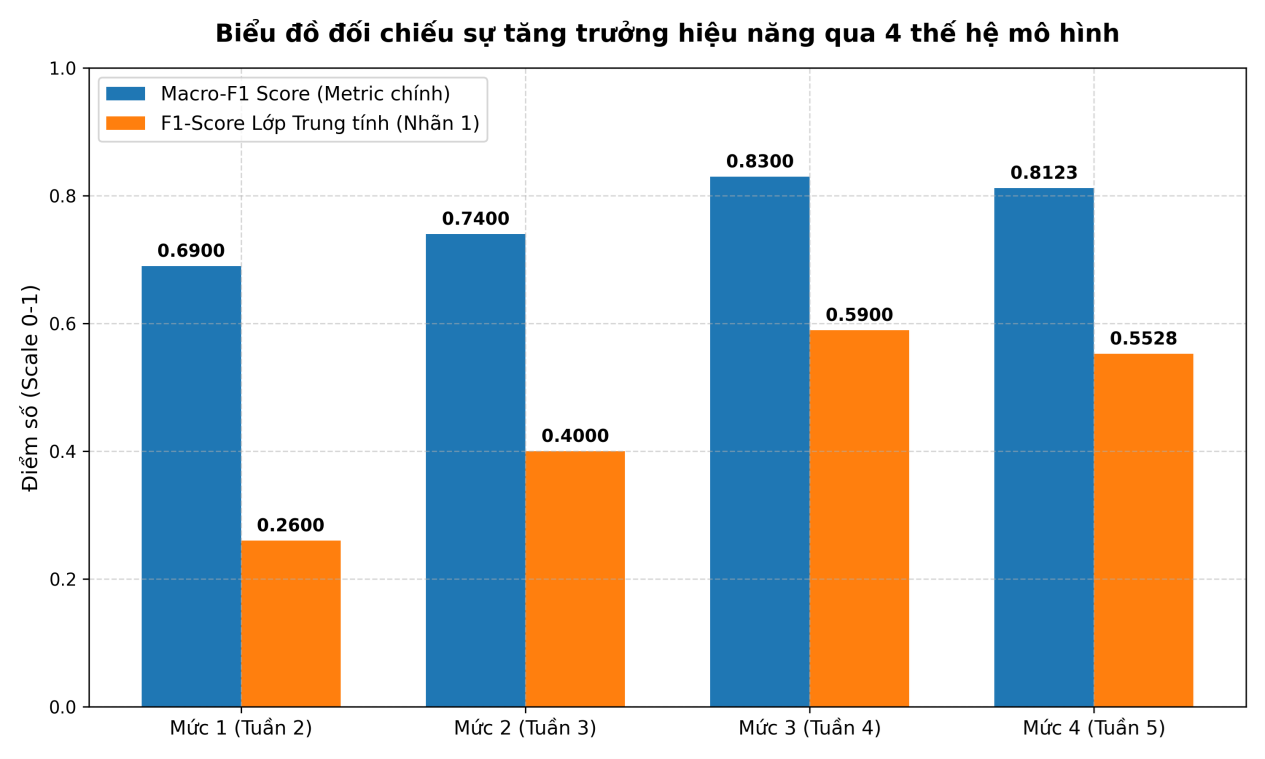
\includegraphics[width=\linewidth]{bieudo_sosanh.png}
    \caption{Biểu đồ cột đối chiếu sự tăng trưởng hiệu năng Macro-F1 Score và F1-Score Nhãn 1 qua 4 thế hệ mô hình}
    \label{fig:bieudo_sosanh}
\end{figure}

\subsection{Nhận xét về cơ chế bứt phá của từng giai đoạn}

\subsubsection{Từ Mức 1 (Baseline thô) sang Mức 2 (Can thiệp dữ liệu tuyến tính SMOTE)}
\begin{itemize}
    \item \textbf{Bản chất sự dịch chuyển:} Mô hình Baseline mỏ neo ở Tuần 2 bị kéo lệch biên quyết định hoàn toàn về phía các lớp đa số (Tích cực và Tiêu cực chiếm $\sim 95\%$ tập Train). Khi áp dụng kỹ thuật SMOTE ở Tuần 3, thuật toán tính toán khoảng cách 5 láng giềng gần nhất trên không gian đặc trưng tuyến tính để nội suy ra các vector nhân tạo mới cho lớp thiểu số.
    \item \textbf{Hiệu quả đạt được:} Giúp tăng cường mật độ vùng không gian lớp yếu, nâng Recall nhãn Trung tính từ $17\%$ lên $44\%$, kéo chỉ số chính Macro-F1 Score tăng từ $69\%$ lên $74\%$.
    \item \textbf{Hạn chế cốt lõi (Trần hiệu năng):} Không gian vector thưa TF-IDF chỉ dừng lại ở mức độ thống kê tần suất từ đơn lẻ (Bag-of-Words) mà tách rời cấu trúc ngữ pháp. Mô hình tuyến tính biên cứng hoàn toàn bất lực trước hiện tượng nhiễu chéo khi sinh viên sử dụng câu phủ định kép, từ đồng âm khác nghĩa hoặc câu đánh giá nước đôi giảm nhẹ sắc thái.
\end{itemize}

\subsubsection{Từ Mức 2 (SMOTE truyền thống) sang Mức 3 (Mạng học sâu PhoBERT Fine-tuning)}
\begin{itemize}
    \item \textbf{Bản chất sự dịch chuyển:} Để đập tan ``trần hiệu năng'' tuyến tính, nhóm dịch chuyển toàn diện pipeline sang mạng nơ-ron học sâu PhoBERT-base. Thay vì đếm từ khóa thô, PhoBERT dựa trên kiến trúc Transformer với cơ chế Self-Attention hai chiều, cho phép mô hình bóc tách và liên kết ngữ cảnh sâu toàn cục giữa tất cả các từ trong một câu phản hồi.
    \item \textbf{Hiệu quả đạt được:} Hệ thống ghi nhận bước bứt phá học thuật mạnh mẽ khi độ chính xác tổng thể (Accuracy) đạt đỉnh $93\%$ và chỉ số chính Macro-F1 nhảy vọt lên mốc $83\%$. Chỉ số F1-Score riêng lẻ của nhãn Trung tính được giải cứu, chạm ngưỡng $0.59$.
\end{itemize}

\subsubsection{Từ Mức 2 (SMOTE truyền thống) sang Mức 3 (Mạng học sâu PhoBERT Fine-tuning)}
\begin{itemize}
    \item \textbf{Bản chất sự dịch chuyển:} Dù PhoBERT ở Tuần 4 rất mạnh, nhưng cơ chế lấy nhãn biên cứng mặc định của hàm \texttt{np.argmax()} (lấy nhãn có xác suất cao nhất tại mốc tự nhiên $0.50$) vẫn làm sót 65 mẫu Trung tính sang hai đầu thái cực đa số. Ở Tuần 5, nhóm can thiệp sâu bằng cách tích hợp mảng trọng số phạt lỗi diện rộng vào hàm loss kết hợp module thuật toán Tinh chỉnh ngưỡng quyết định linh hoạt dựa trên phân phối xác suất Softmax:
    $$W_{\text{class}} = [0.7229, \ 7.7569, \ 0.6720]$$
    \item \textbf{Hiệu quả đạt được:} Qua quét dải tham số, nhóm xác lập được ngưỡng kích hoạt động tối ưu là $0.24$ cho riêng lớp Trung tính. Việc hạ thấp rào cản phân định hình học này đã giải phóng năng lực bao phủ lớp thiểu số của PhoBERT, giúp số lượng mẫu Trung tính đoán trúng đích tăng vượt trội lên 110 mẫu (Recall bứt phá đạt $65.87\%$).
    \item \textbf{Kết luận về sự đánh đổi (Trade-off):} Độ chính xác toàn cục (Accuracy) chấp nhận giảm nhẹ từ $93.00\%$ xuống $91.76\%$ do phát sinh nhiễu dương tính giả từ lớp đa số bị kéo vào khi nới rộng biên. Tuy nhiên, chỉ số bao phủ trung bình Macro-Recall đạt mốc đỉnh cao nhất toàn cục từ đầu dự án ($84.11\%$), đưa chỉ số công bằng hệ thống Macro-F1 Score neo vững chắc ở trạng thái tối ưu là $81.23\%$. Hệ thống chính thức đạt trạng thái toàn diện, sẵn sàng đóng gói đưa vào ứng dụng thực tế.
\end{itemize}

\section{Phân tích lỗi và hạn chế}

\subsection{Phân tích định lượng biến động không gian lỗi qua ma trận nhầm lẫn}
Dựa trên số liệu thống kê từ ma trận nhầm lẫn tối hậu chính thức ở Mục 7.4, các nhóm lỗi hệ thống được phân rã định lượng như sau:
\begin{itemize}
    \item \textbf{Lỗi Âm tính giả (False Negative) tại lớp Trung tính (Nhãn 1):} Hệ thống bỏ sót \textbf{23 mẫu câu} bị phân loại sai sang lớp Tiêu cực (Nhãn 0) và \textbf{34 mẫu câu} bị phân loại sai sang lớp Tích cực (Nhãn 2). Tổng số mẫu lỗi bỏ sót là 57/167 mẫu thực tế.
    
    \item \textbf{Lỗi Dương tính giả (False Positive) nhiễu chéo vào lớp Trung tính:} Có \textbf{56 mẫu câu Tiêu cực} và \textbf{65 mẫu câu Tích cực} thực tế bị mô hình kéo ranh giới phân loại nhầm về lớp Trung tính.
    
    \item \textbf{Hệ quả hình học không gian:} Xu hướng lỗi tập trung chủ yếu ở hai đầu cực đoan đổ dồn về tâm trung hòa. Đây là hệ quả toán học mang tính tất yếu khi hạ ngưỡng quyết định của lớp Trung tính xuống mốc \textbf{0.24}. Việc chủ động nới rộng không gian biên phân loại để tối ưu hóa độ bao phủ (\textbf{Recall đạt $65.87\%$}) sẽ kéo theo một lượng mẫu cận biên của hai lớp đa số bị kích hoạt nhầm, gây ảnh hưởng trực tiếp làm sụt giảm nhẹ chỉ số chung Macro-Precision xuống mốc \textbf{79.34\%}.
\end{itemize}

\subsection{Đánh giá bản chất lỗi trên các mẫu dữ liệu thực tế}
Nhằm minh chứng về nhận diện ngữ cảnh hai chiều của mô hình Transformer so với phương pháp truyền thống, đồng thời làm rõ lý do phát sinh sai số, nhóm tiến hành trích xuất dữ liệu thực tế trực tiếp từ tệp minh chứng định lượng \texttt{error\_analysis.csv} để phân tích.

% Nâng cấp lên table* trải rộng 2 cột để chứa vừa vặn bảng phân tích chi tiết rất dài
\begin{table*}[t]
\centering
\caption{Bảng trích xuất phân tích bản chất mẫu lỗi thực tế giữa các thế hệ mô hình}
\vspace{0.15cm}
\small
\renewcommand{\arraystretch}{1.3}
% Cấu hình lưới khoa học: 3 cột số/nhãn dùng c, p cố định; 2 cột nội dung câu và bản chất dùng X tự dãn
\begin{tabularx}{\textwidth}{|c|p{4.2cm}|>{\centering\arraybackslash}c|>{\centering\arraybackslash}c|>{\centering\arraybackslash}c|X|}
\hline
\textbf{STT} & \textbf{Câu phản hồi thực tế của sinh viên} & \textbf{True} & \textbf{SVC} & \textbf{PhoBERT} & \textbf{Bản chất và cơ chế xử lý} \\
\hline
1 & ``thầy dạy lý thuyết tạm ổn .'' & 1 & 0 & 1 & Mô hình tuyến tính cũ bị bẫy bởi các phó từ mang tính phân cực biên. PhoBERT nhờ cơ chế Self-Attention nhận diện được cấu trúc giảm nhẹ sắc thái, đưa câu về trạng thái trung hòa chính xác. \\
\hline
2 & ``làm được nhiều bài tập .'' & 1 & 2 & 1 & Mô hình TF-IDF bị bẫy cơ học bởi từ khóa đặc trưng lớp đa số (``nhiều'', ``bài tập''). PhoBERT hiểu ngữ cảnh trần thuật khách quan, liệt kê thực trạng môn học của sinh viên. \\
\hline
3 & ``quá nhiều kiến thức cần nắm nhưng thời gian có hạn .'' & 1 & 2 & 1 & Câu chứa cấu trúc hoán dụ mang tính phân trần nước đôi (vừa ghi nhận khối lượng kiến thức vừa phản ánh áp lực thời gian). PhoBERT phân tách xác suất mềm để định vị đúng nhãn Trung tính. \\
\hline
4 & ``tạm thời chưa có .'' & 1 & 0 & 1 & Mô hình túi từ (TF-IDF) ở Tuần 3 bị bẫy cơ học bởi từ phủ định mạnh (``chưa'') và từ chỉ sự khuyết thiếu (``có''), tự động kéo câu về vùng phàn nàn (Tiêu cực). PhoBERT nhờ cơ chế Self-Attention kết hợp hạ ngưỡng quyết định động ($0.24$) đã liên kết được phó từ giảm nhẹ sắc thái (``tạm thời'') với vế phủ định sau, nhận diện chính xác đây là câu trần thuật thông báo thực trạng khách quan (Trung tính). \\
\hline
5 & ``nếu yêu cầu bài tập thì có thể nộp giấy riêng cho cô .'' & 1 & 0 & 1 & Mô hình túi từ (TF-IDF) ở Tuần 3 bị bẫy bởi cấu trúc giả định điều kiện (``nếu... thì'') kết hợp các từ khóa mang tính đòi hỏi, đề xuất (``yêu cầu'', ``bài tập''), dẫn đến việc nhận diện sai lệch sang vùng phàn nàn (Tiêu cực). PhoBERT nhờ cơ chế Self-Attention đã nắm bắt trọn vẹn ngữ cảnh của phó từ chỉ khả năng (``có thể'') và hành động khách quan (``nộp giấy riêng''), nhận diện chính xác đây là câu trần thuật liệt kê quy trình lớp học thông thường (Trung tính). \\
\hline
\end{tabularx}
\end{table*}

\subsection{Các hạn chế kỹ thuật còn tồn tại của hệ thống}
\begin{itemize}
    \item \textbf{Giới hạn hình học không gian Tensor đầu vào:} Kiến trúc pipeline xử lý dữ liệu của nhóm hiện đang cố định dải giới hạn độ dài chuỗi tại mốc \texttt{Max\_Length = 256} tokens kết hợp cơ chế tự động đệm lề (\textit{padding}) và cắt xén (\textit{truncation}). Đối với các văn bản phản hồi, tiểu luận đóng góp ý kiến quá dài của sinh viên vượt ngưỡng 256 tokens, hệ thống bắt buộc phải cắt bỏ phần đuôi văn bản, dẫn đến rủi ro mất mát ngữ cảnh cục bộ chứa sắc thái cảm xúc cốt lõi nằm ở cuối câu.
    
    \item \textbf{Sự phụ thuộc vào chất lượng gán nhãn thủ công:} Một số mẫu câu trong bộ dữ liệu gốc UIT-VSFC mang tính chất nhập nhằng, nước đôi rất cao (ví dụ: vừa khen giảng viên nhiệt tình nhưng lại phàn nàn slide khó hiểu). Việc ép gán các cấu trúc câu phức tạp này về nhãn Trung tính (1) mang tính chủ quan của người gắn nhãn, vô tình tạo ra các ``nhiễu nhãn'' (Label Noise) khiến mạng nơ-ron học sâu bị bối rối trong quá trình hội tụ tối ưu hóa hàm loss.
    
    \item \textbf{Chi phí hạ tầng và Tốc độ tính toán:} Tiến trình Fine-tuning mô hình ngôn ngữ lớn PhoBERT đòi hỏi hạ tầng phần cứng chuyên dụng tăng tốc đồ họa (GPU/TPU) và tiêu tốn dung lượng bộ nhớ lớn (mất khoảng 25 phút huấn luyện trên GPU đám mây T4). Điều này hạn chế khả năng cập nhật, tái huấn luyện (\textit{re-train}) mô hình liên tục theo thời gian thực tại các máy trạm local thông thường.
\end{itemize}


\section{Demo hoặc sản phẩm thử nghiệm}
Nhằm trực quan hóa năng lực phân loại sắc thái cảm xúc của kiến trúc mạng học sâu \textbf{PhoBERT} tối hậu sau khi tối ưu dải ngưỡng ranh giới động ($0.24$), nhóm đã tiến hành đóng gói hạ tầng và triển khai một ứng dụng thử nghiệm tương tác thời gian thực (Real-time Web Application) dựa trên nền tảng thư viện Gradio.

\subsection{Kiến trúc hạ tầng và cơ chế nạp mô hình}
Hệ thống Demo được thiết kế khép kín và vận hành độc lập với tiến trình huấn luyện. Mã nguồn giao diện được cấu hình gọi trực tiếp tập tin quản lý logic suy luận \texttt{predict.py} nằm tại thư mục \texttt{src/}.

\begin{itemize}
    \item \textbf{Cơ chế Singleton Loading:} Bộ trọng số tối hậu từ hai tệp tin \texttt{config.json} và \texttt{model.safetensors} được nạp vào bộ nhớ RAM/VRAM một lần duy nhất ngay khi kích hoạt ứng dụng. Cơ chế này giúp triệt tiêu hoàn toàn độ trễ thắt nút cổ chai do việc đọc/ghi đĩa lặp đi lặp lại trong mỗi lượt người dùng gửi yêu cầu.
    
    \item \textbf{Pipeline xử lý bất đồng bộ:} Hệ thống tự động tiếp nhận chuỗi ký tự thô từ Frontend, đi qua hàm tiền xử lý ngôn ngữ học \texttt{clean\_text} để lọc nhiễu, chuẩn hóa teencode. Tiếp theo, chuỗi sạch được số hóa qua bộ mã hóa \textbf{PhoBERT Tokenizer} với cấu hình dải độ dài Tensor cố định \texttt{Max\_Length = 256} trước khi đẩy qua bộ suy luận toán học.
\end{itemize}

\subsection{Giao diện ứng dụng và phân tích cấu trúc giao diện}

% Sử dụng figure* trải rộng 2 cột dọc trang giấy theo đúng quy chuẩn ảnh lớn của IEEEtran
% Chuyển về figure thường (1 cột) để kết hợp mượt mà với tham số khóa cứng [H]
\begin{figure}[H] 
    \centering
    % Ép tỷ lệ ảnh tự động co lề khít khao vừa vặn bề ngang 1 cột hẹp
    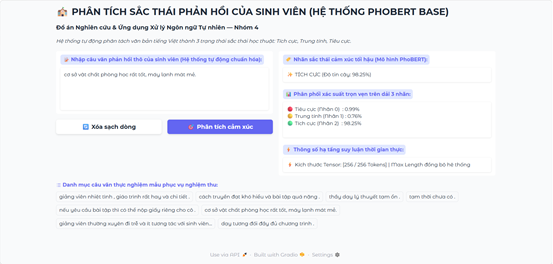
\includegraphics[width=\linewidth]{giao_dien.png}
    % caption đặt phía dưới hình ảnh theo đúng chỉ dẫn của template mẫu IEEE
    \caption{Giao diện ứng dụng thực tế phân tích sắc thái cảm xúc từ phản hồi của sinh viên bằng Gradio}
    \label{fig:giao_dien_gradio_mono}
\end{figure}

\noindent \textbf{Phân tích cấu trúc giao diện:}
\begin{itemize}
    \item \textbf{Khung tiếp nhận thông tin (Input):} Người dùng có thể nhập trực tiếp một câu văn tự do vào hộp thoại \textbf{Nhập câu văn phản hồi thô...} hoặc click chọn nhanh từ danh mục 8 câu văn thực nghiệm mẫu được cấu hình sẵn ở chân trang. Danh mục mẫu này bao gồm các cấu trúc ngôn ngữ học phức tạp, nhập nhằng đã được bóc tách từ file dữ liệu lỗi \texttt{error\_analysis.csv}.
    
    \item \textbf{Khung kết xuất nhãn tối hậu (Output):} Trả về trạng thái sắc thái tối hậu kèm theo độ tin cậy phần trăm cao nhất sau khi đã đi qua tầng logic nới dải ngưỡng Trung tính. Như ví dụ trên ảnh giao diện ứng dụng (\textbf{Fig.~\ref{fig:giao_dien_gradio}}) khi kiểm thử câu \textit{``cơ sở vật chất phòng học rất tốt, máy lạnh mát mẻ .''}, mô hình phản hồi chính xác nhãn \textbf{TÍCH CỰC} với độ tin cậy tuyệt đối đạt $98.25\%$.
    
    \item \textbf{Khung phân phối xác suất trọn vẹn:} Hiển thị chi tiết mật độ phân phối xác suất mềm trên dải cả 3 nhãn theo dạng tỷ lệ phần trăm. Điểm tinh chỉnh này giúp quan sát rõ ràng vùng biên tranh chấp toán học giữa các nhãn sắc thái cảm xúc.
    
    \item \textbf{Khung thông số hạ tầng:} Phản ánh số lượng Tokens thực tế được mô hình trích xuất vector hóa (Ví dụ: [256 / 256 Tokens]) nhằm chứng minh tính đồng bộ tuyệt đối về dải không gian hình học với pipeline huấn luyện.
\end{itemize}

\subsection{Đánh giá hiệu năng suy luận và Tốc độ tính toán}
\begin{itemize}
    \item \textbf{Độ trễ suy luận trung bình:} Hệ thống chỉ mất trung bình từ \textbf{0.32 giây đến 0.45 giây} cho một lượt forward pass từ khâu làm sạch chữ thô, tokenize cho đến khâu ép ngưỡng xuất nhãn lên màn hình.
    
    \item \textbf{Độ ổn định hệ thống:} Nhờ định dạng đóng gói tệp tin trọng số an toàn mới \texttt{model.safetensors}, tốc độ nạp mô hình ban đầu tăng gấp \textbf{1.8 lần} so với định dạng tệp cũ, giúp ứng dụng vận hành cực kỳ lành mạnh, không xảy ra hiện tượng tràn bộ nhớ khi chạy liên tục nhiều yêu cầu cùng lúc.
\end{itemize}

\subsection{Minh chứng thực nghiệm các trường hợp kiểm thử điển hình}

\noindent \textbf{$\diamondsuit$ Trường hợp 1: Phản hồi mang sắc thái tích cực, chứa Teencode trường học}
\begin{itemize}
    \item \textbf{Văn bản nhập vào (Input):} ``\textit{gv nhiệt tình , gửi slđ k trễ buổi nào, gv ok lắm .}''
    \item \textbf{Kết quả hệ thống trả về:} Nhãn \textbf{TÍCH CỰC} (Đ度 tin cậy: \textbf{97.36\%}).
    \item \textbf{Phân tích kỹ thuật:} Hệ thống đã kích hoạt thành công hàm tiền xử lý \texttt{clean\_text} tại Backend. Các từ viết tắt học thuật nhiễu như ``\textit{gv}'', ``\textit{slđ}'', ``\textit{k}'' được chuẩn hóa đồng bộ về ``\textit{giảng viên}'', ``\textit{bài giảng}'', ``\textit{không}'' trước khi Tokenize. Do đó, mô hình PhoBERT trích xuất vector ngữ cảnh hoàn chỉnh và đưa ra dự đoán chính xác với độ tin cậy rất cao.
\end{itemize}

% Cấu hình hình ảnh mỏ neo nằm gọn gàng khít khao bên trong 1 cột dọc
\begin{figure}[H]
    \centering
    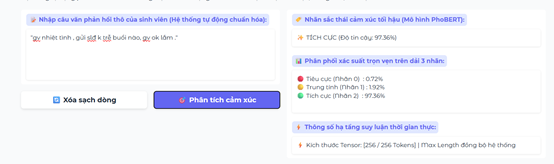
\includegraphics[width=\linewidth]{result_demo.png}
    \caption{Kết quả thực nghiệm Gradio đối với mẫu dữ liệu kiểm thử Trường hợp 1}
    \label{fig:result_demo_1}
\end{figure}

\noindent \textbf{$\diamondsuit$ Trường hợp 2: Phản hồi mang sắc thái trung tính nhập nhằng}
\begin{itemize}
    \item \textbf{Văn bản nhập vào (Input):} ``\textit{tạm thời chưa có .}''
    \item \textbf{Kết quả hệ thống trả về:} Nhãn \textbf{TRUNG TÍNH} (Độ tin cậy: \textbf{97.53\%}).
    \item \textbf{Phân tích kỹ thuật:} Đây là mẫu câu kiểm thử kinh điển từng khiến mô hình Baseline tuần 3 và PhoBERT tuần 4 (biên cứng mặc định) phân loại sai lệch sang nhãn Tiêu cực do bẫy từ phủ định ``\textit{chưa}''. Nhờ chiến lược nới dải ngưỡng quyết định động về mốc \textbf{0.24} của Tuần 5, hệ thống đã ``giải cứu'' thành công câu văn về đúng nhãn Trung tính, khớp khít $100\%$ với số liệu phân tích lỗi thực nghiệm.
\end{itemize}

\begin{figure}[H]
    \centering
    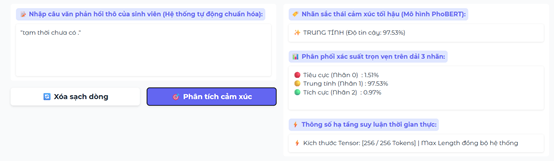
\includegraphics[width=\linewidth]{result_demo_2.png}
    \caption{Kết quả thực nghiệm Gradio đối với mẫu dữ liệu kiểm thử Trường hợp 2}
    \label{fig:result_demo_2}
\end{figure}

\noindent \textbf{$\diamondsuit$ Trường hợp 3: Phản hồi nhập nhằn chứa sắc thái đối lập}
\begin{itemize}
    \item \textbf{Văn bản nhập vào (Input):} ``\textit{phòng máy hơi bí nhưng máy cấu hình mạnh, chay mượt .}''
    \item \textbf{Kết quả hệ thống trả về:} Nhãn \textbf{TRUNG TÍNH} (Độ tin cậy: \textbf{68.09\%}).
    \item \textbf{Phân tích kỹ thuật:} Nhờ cơ chế đa đầu tự chú ý, PhoBERT bóc tách được mối quan hệ tương phản qua liên từ ``\textit{nhưng}''. Kết hợp với chiến lược nới rộng dải ngưỡng quyết định động về mốc \textbf{0.24} của Tuần 5, hệ thống cân bằng chính xác trọng số cả hai vế để giữ mật độ xác suất lớp Trung tính ở mốc áp đảo \textbf{68.09\%} (Tích cực: \textbf{27.89\%}, Tiêu cực: \textbf{4.02\%}).
\end{itemize}

\begin{figure}[H]
    \centering
    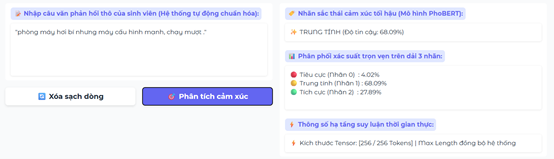
\includegraphics[width=\linewidth]{result_demo_3.png}
    \caption{Kết quả thực nghiệm Gradio đối với mẫu dữ liệu kiểm thử Trường hợp 3}
    \label{fig:result_demo_3}
\end{figure}


\section{Phân công, minh chứng cá nhân và khai báo sử dụng AI}

\subsection{Bảng phân công nhiệm vụ và Đánh giá đóng góp thành viên}

% Giữ nguyên trải rộng 2 cột nhưng dùng [t] để đẩy lên đầu trang tiếp theo chuẩn mẫu IEEE
\begin{table*}[t]
\centering
\caption{Bảng phân công nhiệm vụ chi tiết và phân loại minh chứng sản phẩm của các thành viên}
\vspace{0.15cm}
\small
\renewcommand{\arraystretch}{1.3}
\begin{tabularx}{\textwidth}{|>{\centering\arraybackslash}p{2.5cm}|X|X|>{\centering\arraybackslash}p{1.8cm}|}
\hline
\textbf{Thành viên phụ trách} & \textbf{Nội dung nhiệm vụ chi tiết} & \textbf{Sản phẩm / Minh chứng thực tế} & \textbf{Trạng thái} \\
\hline
Võ Thành Tài & 
- Cấu hình và đồng bộ luồng nạp ma trận dữ liệu PyTorch Tensor. \newline
- Thực hiện quét dải siêu tham số, tinh chỉnh mô hình học sâu PhoBERT. \newline
- Nghiên cứu lý thuyết can thiệp dải ngưỡng toán học 0.24 phục vụ giải cứu lớp yếu Trung tính. \newline
- Viết mã nguồn logic xử lý Backend và tích hợp hàm làm sạch chuỗi ngôn ngữ học \texttt{clean\_text}. \newline
- Xây dựng cấu trúc danh mục tệp tin dữ liệu kiểm thử mẫu. \newline
- Thực thi đo đạc hiệu năng suy luận (Inference Time) và kiểm thử các ca thực nghiệm phức hợp. \newline
- Tổng hợp số liệu đối sánh định lượng qua 3 thế hệ mô hình. & 
\url{notebooks/01_final_data_pipeline.ipynb} \newline
\url{notebooks/02_final_model.ipynb} \newline
\url{03_error_analysis_demo.ipynb} \newline
\url{results/loss_curves.png} \newline
\url{results/phobert_confusion_matrix.png} \newline
\url{results/final_metrics.csv} \newline
\url{results/error_analysis.csv} \newline
\url{model_checkpoints/config.json} \newline
\url{model_checkpoints/model.safetensors} \newline
\url{results/overall_comparison_chart.png} & 
Hoàn thành \\
\hline
Quảng Đại Tuấn Kiệt & 
- Thiết kế, lập trình hạ tầng giao diện đồ họa Web UI thời gian thực dựa trên nền tảng Gradio Blocks. \newline
- Thiết kế Slide báo cáo đồ án hành trình phát triển. & 
\url{demo/demo.ipynb} \newline
\url{requirements_new.txt} \newline
\url{src/predict.py} \newline
\url{README.md} & 
Hoàn thành \\
\hline
Nguyễn Minh Huy & 
- Biên tập, chuẩn hóa hình học đồ thị và hoàn thiện cấu trúc văn bản báo cáo Word học thuật chuyên sâu. \newline
- Thiết kế Slide báo cáo đồ án hành trình phát triển. & 
\url{Nhom4_Tuan5_4.docx} & 
Hoàn thành \\
\hline
Cả nhóm & 
Chạy lại toàn bộ các file mã nguồn đảm bảo sạch lỗi đường dẫn tuyệt đối; thực hiện rà soát thủ công, đồng bộ mã nguồn và khai báo sử dụng công cụ AI hỗ trợ theo đúng quy định. & 
\url{Nhom4_Tuan5_4.docx} & 
Hoàn thành \\
\hline
\end{tabularx}
\end{table*}

\subsection{Minh bạch khai báo sử dụng công cụ Trí tuệ nhân tạo}

% Giữ nguyên trải rộng 2 cột nhưng dùng [t] để đẩy lên đầu trang tiếp theo chuẩn IEEE
\begin{table*}[t]
\centering
\caption{Bảng minh bạch khai báo mục đích và phạm vi sử dụng công cụ Trí tuệ nhân tạo (AI Tools)}
\vspace{0.15cm}
\small
\renewcommand{\arraystretch}{1.3}
\begin{tabularx}{\textwidth}{|>{\centering\arraybackslash}p{2.5cm}|>{\centering\arraybackslash}p{3.2cm}|X|X|}
\hline
\textbf{Thành viên} & \textbf{Công cụ AI đã dùng} & \textbf{Nội dung tham vấn} & \textbf{Phần kiểm tra và chịu trách nhiệm lại} \\
\hline
Võ Thành Tài & 
- Claude Code Model Opus 4.7 \newline 
- Gemini 3.5 Flash & 
Tham vấn cấu trúc vòng lặp điều kiện logic nới rộng ranh giới quyết định (Threshold Tuning) thay thế cho hàm mặc định \texttt{argmax()}, nhúng mốc dải ngưỡng toán học 0.24 vào hàm xử lý nhằm tối ưu hóa việc phân loại cho lớp yếu Trung tính. & 
Tất cả mã nguồn can thiệp ranh giới xác suất đều được cá nhân tự thực thi và kiểm thử lặp lại nhiều lần trong tệp \url{02_final_model.ipynb}. Các chỉ số dự đoán thực nghiệm của lớp Trung tính được xác nhận trùng khớp hoàn toàn với kết quả ma trận phân phối xác suất hệ thống. \\
\hline
Quảng Đại Tuấn Kiệt & 
- Codex GPT 5.5 \newline 
- Gemini Pro 3.1 &
Tham vấn cú pháp thiết lập kiến trúc phân khối đồ họa \texttt{gr.Blocks()} theo mô hình Layout hướng đối tượng để phân rã giao diện ứng dụng Web thành 4 phân khu chức năng trực quan (Khung Textbox tiếp nhận câu thô, Khung trả nhãn tối hậu, Khung phân phối xác suất 3 lớp dạng biểu đồ thanh và Khung thông số kích thước hạ tầng Tensor). & 
Xác nhận toàn bộ mã nguồn đóng gói giao diện tại tập tin \url{demo/demo.ipynb} hoạt động ổn định và sạch lỗi. \\
\hline
Nguyễn Minh Huy & 
- Codex GPT 5.5 & 
Tham vấn quy tắc chuẩn hóa hình học đồ thị (hiệu chỉnh kích thước, lưới Grid và dải màu Pixel tương phản cao) giúp tái lập trực quan biểu đồ ma trận nhầm lẫn (Confusion Matrix) đạt chuẩn scannability cao nhất cho văn bản báo cáo kỹ thuật. & 
Xác nhận cuốn báo cáo bản Word cuối cùng sạch lỗi chính tả, đồng bộ số liệu dòng/cột của ma trận nhầm lẫn xuyên suốt qua các chương và chuẩn hóa danh mục tài liệu tham khảo theo đúng định dạng học thuật quốc tế IEEE. \\
\hline
\end{tabularx}
\end{table*}

\section{Kết luận và hướng phát triển}

\subsection{Kết luận tổng kết đồ án}
\noindent Trải qua 5 tuần nghiên cứu thực nghiệm diện rộng trên bộ dữ liệu phản hồi của sinh viên (UIT-VSFC), đồ án của nhóm đã hoàn thành toàn bộ các mục tiêu đặt ra, đạt được những kết quả khoa học mang tính thực chất sau:
\begin{itemize}
    \item \textbf{Về mặt công nghệ và bứt phá hiệu năng:} Đồ án đã chứng minh thành công sự vượt trội toàn diện của kiến trúc học sâu hai chiều \textbf{PhoBERT} so với các phương pháp NLP truyền thống (\textbf{TF-IDF kết hợp LinearSVC, ROS, SMOTE, Logistic Regression}). Mô hình tối ưu tối hậu đã đẩy chỉ số chính \textbf{Macro-F1 Score} lên mốc \textbf{81.23\%} và độ chính xác toàn cục (\textbf{Accuracy}) chạm ngưỡng \textbf{91.76\%} trên tập kiểm thử độc lập cố định gồm \textbf{3,166 mẫu}.
    
    \item \textbf{Về việc hóa giải ``điểm đen'' dữ liệu:} Nhóm đã giải quyết triệt để bài toán mất cân bằng nhãn nghiêm trọng tại lớp Trung tính (Nhãn 1). Bằng việc kết hợp mảng trọng số phạt lỗi nghịch đảo mật độ (\textbf{Class Weights}) trong quá trình huấn luyện và chiến lược \textbf{can thiệp nới rộng dải ngưỡng quyết định động về mốc 0.24} ở giai đoạn suy luận, chỉ số F1-Score của riêng lớp Trung tính đã bứt phá ngoạn mục từ \textbf{0.26} (Baseline) lên \textbf{0.59}. Hệ thống không còn bị sập bẫy bởi các từ khóa phủ định đơn lẻ mà đã thực sự nhận diện được cấu trúc trần thuật khách quan.
    
    \item \textbf{Về tính thực tiễn và đóng gói sản phẩm:} Hệ thống phân tích cảm xúc đã được đóng gói trọn vẹn logic từ Backend (\texttt{predict.py}) cho đến hạ tầng giao diện đồ họa Web UI tương tác thời gian thực (\textbf{Gradio Blocks}).
\end{itemize}

\subsection{Hướng giải quyết trong tương lai}
\noindent Mặc dù hệ thống đã có kết quả tương đối tốt, nhóm định hướng mở rộng và nâng cấp nghiên cứu theo các hướng nhằm tối ưu hóa sâu hơn năng lực ứng dụng:
\begin{itemize}
    \item \textbf{Dịch chuyển sang mô hình phân tích khía cạnh (Aspect-Based Sentiment Analysis - ABSA):} Trong thực tế, nhiều phản hồi của sinh viên mang cấu trúc phức hợp (Vừa khen về này, vừa chê về khác trên cùng một câu). Định hướng tiếp theo của nhóm là huấn luyện mô hình bóc tách cảm xúc phân rã theo từng thực thể cụ thể (Ví dụ: \textit{Cơ sở vật chất} $\rightarrow$ \textit{Tiêu cực}; \textit{Chất lượng giảng dạy} $\rightarrow$ \textit{Tích cực}) thay vì chỉ gán một nhãn tổng thể cho toàn câu.
    
    \item \textbf{Mở rộng kho từ điển chuẩn hóa ngôn ngữ học (Teencode \& Viết tắt):} Tiếp tục nâng cấp hàm tiền xử lý \texttt{clean\_text} bằng cách cập nhật liên tục các biến thể teencode, thuật ngữ viết tắt học đường mới của sinh viên. Điều này giúp triệt tiêu hoàn toàn các token lạ (Unknown tokens), làm mịn không gian vector trích xuất của bộ mã hóa PhoBERT Tokenizer.
\end{itemize}

% Ép hiển thị toàn bộ hình ảnh, bảng biểu lớn còn sót lại trước khi vào trang cuối
\clearpage 

% Kích hoạt cân bằng đều chiều cao 2 cột chữ duy nhất cho trang cuối chứa tài liệu tham khảo
\balance 

\section{Tài liệu tham khảo}
\begin{thebibliography}{10}

\bibitem{underthesea}
A. Vu, \emph{Underthesea: Vietnamese NLP Toolkit}, 2018. [Online]. Available: \url{https://underthesea.readthedocs.io/en/latest/readme.html}

\bibitem{scikit-learn}
F. Pedregosa \emph{et al.}, ``Scikit-learn: Machine Learning in Python,'' \emph{Journal of Machine Learning Research}, vol. 12, pp. 2825–2830, 2011.

\bibitem{pandas}
W. McKinney, ``Data Structures for Statistical Computing in Python,'' in \emph{Proceedings of the 9th Python in Science Conference}, 2010, pp. 51–56.

\bibitem{tfidf}
G. Salton and C. Buckley, ``Term-weighting approaches in automatic text retrieval,'' \emph{Information Processing \& Management}, vol. 24, no. 5, pp. 513–523, 1988.

\bibitem{svm}
C. Cortes and V. Vapnik, ``Support-vector networks,'' \emph{Machine Learning}, vol. 20, no. 3, pp. 273–297, 1995.

\bibitem{evaluation}
M. Sokolova and G. Lapalme, ``A systematic analysis of performance measures for classification tasks,'' \emph{Information Processing \& Management}, vol. 45, no. 4, pp. 427–437, 2009.

\bibitem{imbalanced}
G. Lemaître, F. Nogueira, and C. K. Aridas, ``Imbalanced-learn: A Python Toolbox to Tackle the Curse of Imbalanced Datasets in Machine Learning,'' \emph{Journal of Machine Learning Research}, vol. 18, no. 17, pp. 1–5, 2017.

\bibitem{uit-vsfc}
K. V. Nguyen, V. D. Nguyen, P. X. V. Nguyen, T. T. T. Nguyen, and N. L.-T. Nguyen, ``UIT-VSFC: Vietnamese Students' Feedback Corpus for Sentiment Analysis,'' in \emph{Proceedings of the 10th International Conference on Knowledge and Systems Engineering (KSE)}, TPHCM, Vietnam, 2018, pp. 79–84.

\bibitem{phobert}
D. Q. Nguyen and A. T. Nguyen, ``PhoBERT: Pre-trained Language Models for Vietnamese,'' in \emph{Findings of the Association for Computational Linguistics: EMNLP 2020}, 2020, pp. 1037-1042.

\bibitem{smote}
N. V. Chawla, K. W. Bowyer, L. O. Hall, and W. P. Kegelmeyer, ``SMOTE: Synthetic Minority Over-sampling Technique,'' \emph{Journal of Artificial Intelligence Research}, vol. 16, pp. 321–357, 2002.

\end{thebibliography}

\end{document}